\section{Pre-process}
This work aim to use the hierarchical Stochastic Block Model (hSBM) described before. Data considered in this work have $\sim 11000$ samples as documents and $\sim 60000$ genes as words ($\sim 20000$ if considering only protein coding genes). In comparison in the original paper~\cite{gerlach2018network} $63$ Wikipedia articles were considered along with $3140$ words. The great amount of data requires some tricks to filter the network and make the computation faster.
Different approaches were tested to pre-processing the data, all of them involving the quantities defined in~\ref{ch:structure}. The goal is to identify components which are able to best separate the realizations or isolate the most interesting genes. 
\paragraph{Low occurrence genes} were selected firstly to approach topic modelling. A $0.5$ threshold was set on occurrence. This method selects genes that appears (have expression greater than zero) only in less than half samples. This approach has some limitations, for instance it doesn't consider genes that appear everywhere (with occurrence $\simeq 1$) but changes their behaviour across realizations.

\paragraph{tf-idf (term frequency–inverse document frequency)} should help. This approach doesn't take in account original expression values $n_{ij}$, but a transformed version
\[
n^{new}_{ij}=\frac{n_{i j}}{M_j}\times \left(1-Log\left(o_i\right)\right)
\] which increases the importance of components with small occurrence $o_i$. This approach doesn't actually select components, which is still an issue.

\paragraph{Highly variable} genes can be selected. This is done using the $CV^2$ analysis done in chapter~\ref{ch:scalinglaws}.
\begin{figure}[htb!]
    \centering
    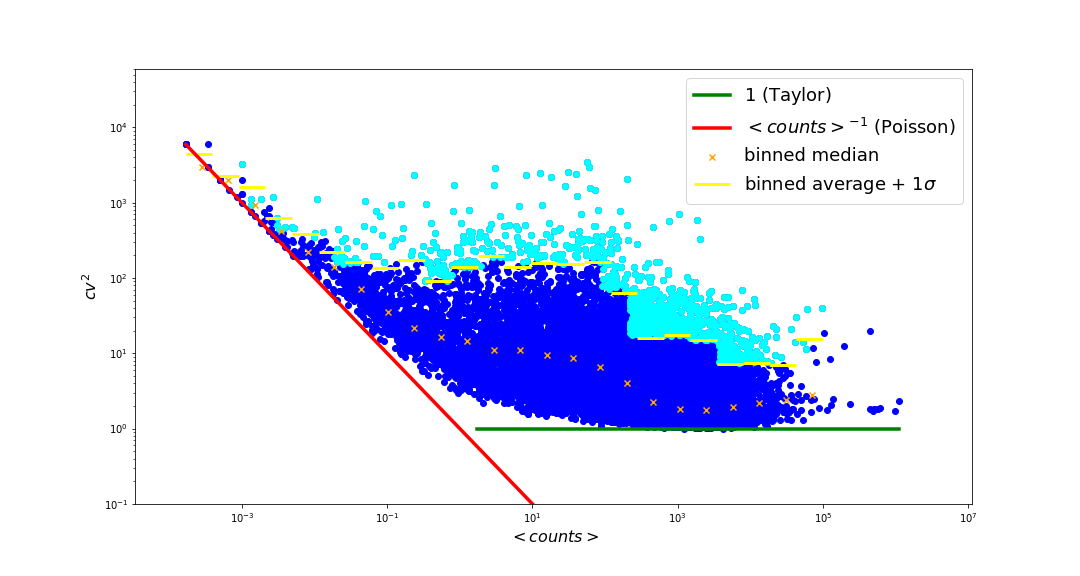
\includegraphics[width=0.8\linewidth]{pictures/topic/cvmean_oversigma.png}
    \caption{Highly variable genes. In cyan genes that are $1 \sigma$ over the average of their bin.}
    \label{fig:topic/cvmean_oversigma}
\end{figure}
Plotting the coefficient of variation versus the mean for each component reveals which components have higher variance with respect to components which, on average, have a similar behaviour. Binned averages and variances were estimated, and only genes with a $CV^2$ over a $\sigma$ greater than the bin's mean were considered. This method seems to select useful genes even if the binned average bound is quite noisy.

\paragraph{Distance from boundaries} can be a similar and alternative method to select highly variable genes. In this case the bound is smooth and well-defined.
\begin{figure}[htb!]
    \centering
    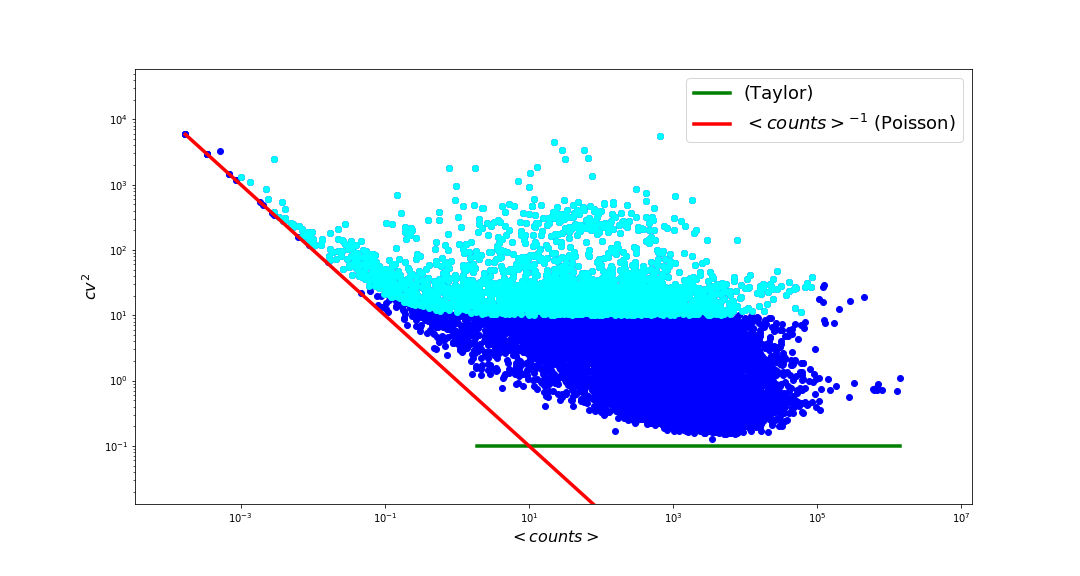
\includegraphics[width=0.8\linewidth]{pictures/topic/cvmean_oversampling.png}
    \caption{In cyan genes which distance from boundaries is greater than $10 CV^2$.}
    \label{fig:topic/cvmean_oversampling}
\end{figure}
The distribution as discussed in~\ref{ch:scalinglaws} have a Poisson-like and a Taylor-like boundaries. So can be considered only components that are the most distant from these boundaries. Moreover, this boundaries can be found with a simple null model, as shown in figure~\ref{fig:scalinglaws/gtex/cvmean_loglog_sampling} the sampling model defines the lower bound of the data.

The last two approaches are the ones which lead to better results, in the following sections gene selection was done by getting only highly variables genes.
In order to reduce the number of documents, samples are picked up from a subset of all the available tissues.